%%%%%%%%%%%%%%%%%%%%%%%%%%%%%%%%%%%%%%%%%%%%%%%%%%%%%%%%%%%%%%%%%%%%%%%%%%%

\documentclass[a4paper,oneside,12pt]{article}
\usepackage{mystyle}

\begin{document}

\title{\Large\bf Cartesian coordinate system}
\author{%%
  Minh Van Nguyen \\
  \url{mvngu@gmx.com}
}
\date{\today}
\maketitle


%%%%%%%%%%%%%%%%%%%%%%%%%%%%%%%%%%%%%%%%%%%%%%%%%%%%%%%%%%%%%%%%%%%%%%%%%%%

\section{Coordinates}

Let's start by discussing how a pair of numbers can be represented as
a picture.  You know that any real number can be represented as a
point on the number line.  \Figure{fig:real_number_line} shows the
irrational numbers $\sqrt{2}$, $e$, and $\pi$ as points on the number
line.  What if you have a pair $\tuple{a}{b}$ of real numbers?  How
would $\tuple{a}{b}$ be represented as a point on the number line?

\begin{figure}[!htbp]
\centering
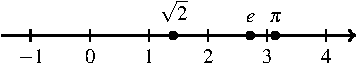
\includegraphics[scale=1.1]{image/03/number-line.pdf}
\caption{%%
  Elements from the set $\RR$ of real numbers can be represented as
  points on the number line.
}
\label{fig:real_number_line}
\end{figure}

The answer is that a pair $\tuple{a}{b}$ of real numbers cannot be
represented as a point on the number line.  You must somehow extend
the number line.  One way to extend the number line is to draw a
vertical line through the point $0$ such that the vertical line is
perpendicular to the number line.  What you then obtain is the
\emph{Cartesian coordinate system} as shown in
\Figure{fig:Cartesian_coordinate_system}.  In the Cartesian coordinate
system, a pair $\tuple{a}{b}$ of real numbers can be represented as a
point with the pair $\tuple{a}{b}$ being now called a pair of
\emph{coordinates}.  The number $a$ in the coordinates $\tuple{a}{b}$
is called the $x$-coordinate because starting from $0$ on the
$x$-axis you must move a horizontal distance of $a$ units to get to
the coordinates $\tuple{a}{0}$.  The number $b$ in the coordinates
$\tuple{a}{b}$ is called the $y$-coordinate because starting from $0$
on the $y$-axis you must move a vertical distance of $b$ units to get
to the coordinates $\tuple{0}{b}$.  Add the coordinates $\tuple{a}{0}$
and $\tuple{0}{b}$ together and you get the coordinates
$\tuple{a}{b}$, which can be drawn as a point in the Cartesian
coordinate system.  The special coordinates $\tuple{0}{0}$ is called
the \emph{origin}.  If $\tuple{a}{b}$ is a pair of coordinates in the
Cartesian coordinate system, you also refer to $\tuple{a}{b}$ as a
point in the Cartesian coordinate system.

\begin{figure}[!htbp]
\centering
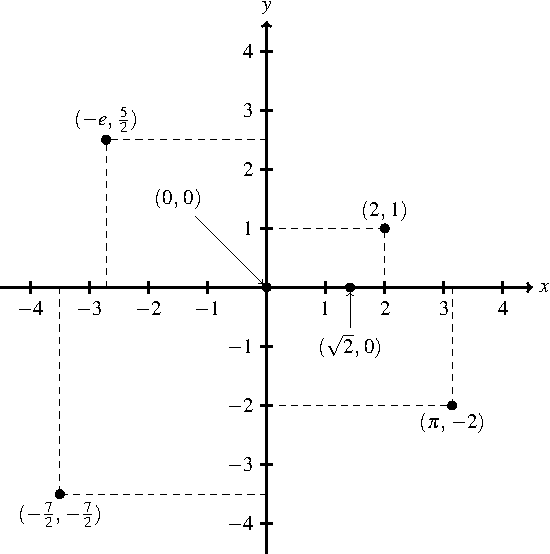
\includegraphics[scale=1.1]{image/03/cartesian-coordinate.pdf}
\caption{%%
  The Cartesian coordinate system consists of two perpendicular axes
  called the $x$-axis and the $y$-axis.  A pair $\tuple{a}{b}$ of real
  numbers can be represented as a point.  Starting from the origin
  $\tuple{0}{0}$, you move a distance of $a$ units along the
  horizontal axis and then move $b$ units along the vertical axis.
  Where you end up is the point $\tuple{a}{b}$.
}
\label{fig:Cartesian_coordinate_system}
\end{figure}

\begin{exercise}
Represent the pairs $\tuple{2}{4}$, $\tuple{0}{-3}$, and
$\tuple{-4}{0}$ as points in the Cartesian coordinate system.
\end{exercise}

\ifbool{showSolution}{
\begin{solution}
See \Figure{fig:some_points_in_Cartesian_coordinate_system}.
%%
\begin{figure}[!htbp]
\centering
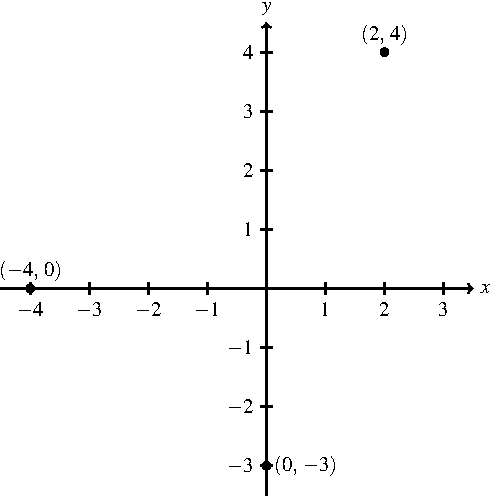
\includegraphics[scale=1.1]{image/03/cartesian-coordinate_2-5_0-3_4-0.pdf}
\caption{%%
  The pairs $\tuple{2}{4}$, $\tuple{0}{-3}$, and $\tuple{-4}{0}$ as
  points in the Cartesian coordinate system.
}
\label{fig:some_points_in_Cartesian_coordinate_system}
\end{figure}
\end{solution}
}{}


%%%%%%%%%%%%%%%%%%%%%%%%%%%%%%%%%%%%%%%%%%%%%%%%%%%%%%%%%%%%%%%%%%%%%%%%%%%

\section{Distance}

The distance between two points $A$ and $B$ is the length of the
straight line from $A$ to $B$.  In the Cartesian coordinate system,
you use the same technique to measure the distance between two
points.  Suppose the points $A$ and $B$ have coordinates
$A = \tuple{x_1}{y_1}$ and $B = \tuple{x_2}{y_2}$; see
\Figure{fig:distance_between_two_points}.  Then there is a third point
$C$ with coordinates $C = \tuple{x_1}{y_2}$.  The line segments $AC$,
$BC$, and $AB$ are the three sides of a right-angled triangle.  The
segment $AC$ has length
\[
a
=
\absoluteValue{y_1 - y_2}
=
\absoluteValue{y_2 - y_1}
\]
and the segment $BC$ has length
\[
b
=
\absoluteValue{x_2 - x_1}
=
\absoluteValue{x_1 - x_2}
\]
but you do not yet know the length of the segment $AB$.  However,
since the points $\triple{A}{B}{C}$ are the three corners of a
right-angled triangle, you can use Pythagoras' theorem to determine
the length of the segment $AB$.

\begin{theorem}
\textbf{Pythagoras' theorem.}
Let $\triple{a}{b}{c}$ be the lengths of the three sides of a
right-angled triangle, where $c$ is the length of the hypotenuse.
Then $c$ can be written as $a^2 + b^2 = c^2$.
\end{theorem}

\begin{figure}[!htbp]
\centering
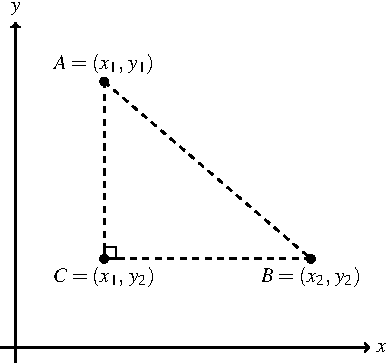
\includegraphics[scale=1.1]{image/03/distance-two-points.pdf}
\caption{%%
  Any two distinct points $A$ and $B$ are two corners of a
  right-angled triangle.  The line segment $AB$ is the hypotenuse,
  whose length can be measured by Pythagoras' theorem.
}
\label{fig:distance_between_two_points}
\end{figure}

Let $c$ be the length of the segment $AB$ in
\Figure{fig:distance_between_two_points}.  Use Pythagoras' theorem to
write
%%
\begin{align*}
c^2
&=
a^2 + b^2 \\[4pt]
&=
\absoluteValue{y_2 - y_1}^2 + \absoluteValue{x_2 - x_1}^2 \\[4pt]
&=
(y_2 - y_1)^2 + (x_2 - x_1)^2.
\end{align*}
%%
Solve the last expression for $c$ and you obtain
\[
c
=
\sqrt{
  (y_2 - y_1)^2
  +
  (x_2 - x_1)^2
}
\]
which proves the following theorem.

\begin{theorem}
\label{thm:distance_between_two_points}
\textbf{Distance.}
Let $A = \tuple{x_1}{y_1}$ and $B = \tuple{x_2}{y_2}$ be two points in
the Cartesian coordinate system.  The distance between $A$ and $B$ can
be written as
\[
\sqrt{
  (y_2 - y_1)^2
  +
  (x_2 - x_1)^2
}.
\]
\end{theorem}

\begin{exercise}
Consider the points $(\sqrt{2}\comma 0)$ and $\tuple{2}{1}$ from
\Figure{fig:Cartesian_coordinate_system}.  Determine the distance
between those two points.
\end{exercise}

\ifbool{showSolution}{
\begin{solution}
Use \Theorem{thm:distance_between_two_points} to write
%%
\begin{align*}
\sqrt{
  (1 - 0)^2
  +
  (2 - \sqrt{2})^2
}
&=
\sqrt{
  1^2 + (2 - \sqrt{2})^2
} \\[4pt]
&\approx
1.3431
\end{align*}
%%
correct to four decimal places.  The symbol ``$\approx$'' means
``approximately''.  In other words, the distance between the points
$(\sqrt{2}\comma 0)$ and $\tuple{2}{1}$ is approximately $1.3431$.
\end{solution}
}{}

\begin{exercise}
Let $\tuple{a}{b}$ be any point in the Cartesian coordinate system.
Calculate the distance from $\tuple{a}{b}$ to the origin.
\end{exercise}

\ifbool{showSolution}{
\begin{solution}
Use \Theorem{thm:distance_between_two_points} to write
%%
\begin{align*}
\sqrt{
  (a - 0)^2 + (b - 0)^2
}
&=
\sqrt{
  a^2 + b^2
}
\end{align*}
%%
which is the distance from the origin to $\tuple{a}{b}$.
\end{solution}
}{}


%%%%%%%%%%%%%%%%%%%%%%%%%%%%%%%%%%%%%%%%%%%%%%%%%%%%%%%%%%%%%%%%%%%%%%%%%%%

\section{Reflection}

Let $\tuple{a}{b}$ be any point in the Cartesian coordinate system.
You can do a number of basic geometric operations on $\tuple{a}{b}$ by
multiplying $a$ or $b$ by $-1$.  For example, imagine you place a
mirror along the $x$-axis.  Then the reflection of $\tuple{a}{b}$ with
respect to the $x$-axis is $\tuple{a}{-1 \times b} = \tuple{a}{-b}$.
If you now place a mirror along the $y$-axis, the reflection of
$\tuple{a}{b}$ with respect to the $y$-axis is
$\tuple{-1 \times a}{b} = \tuple{-a}{b}$.  Multiplying each of $a$ and
$b$ by $-1$ and you get $\tuple{-a}{-b}$, which is the diagonal
reflection of $\tuple{a}{b}$.  See \Figure{fig:reflections_of_point}
for an example.

\begin{figure}[!htbp]
\centering
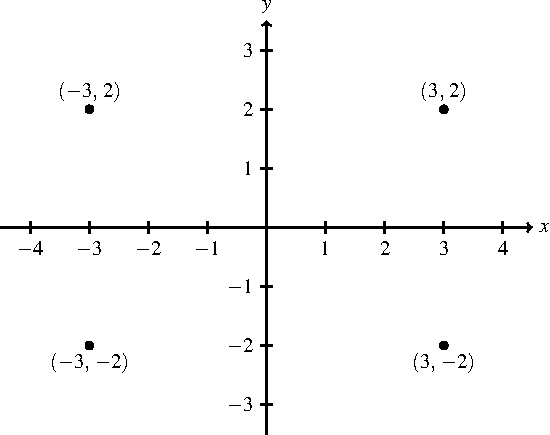
\includegraphics[scale=1.1]{image/03/reflection.pdf}
\caption{%%
  Some reflections of the point $\tuple{3}{2}$.  The point
  $\tuple{3}{2}$ together with its three reflections form the four
  corners of a rectangle.  The centre of the rectangle is the origin
  $\tuple{0}{0}$.
}
\label{fig:reflections_of_point}
\end{figure}

\begin{exercise}
Consider the point $A = \tuple{-2}{4}$.  Determine the reflections of
$A$ with respect to the $x$- and $y$-axes and also the diagonal
reflection of $A$.
\end{exercise}

\ifbool{showSolution}{
\begin{solution}
See \Figure{fig:reflections_of_m2_4}.  The reflection of $A$ with
respect to the $x$-axis is $\tuple{-2}{-4}$.  The reflection of $A$
with respect to the $y$-axis is $\tuple{2}{4}$.  The diagonal
reflection is $\tuple{2}{-4}$.
%%
\begin{figure}[!htbp]
\centering
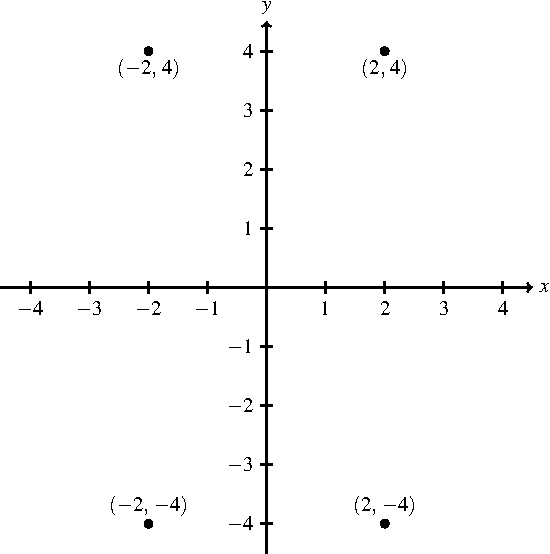
\includegraphics[scale=1.1]{image/03/reflection-eg.pdf}
\caption{%%
  Reflections of the point $\tuple{-2}{4}$.
}
\label{fig:reflections_of_m2_4}
\end{figure}
\end{solution}
}{}


%%%%%%%%%%%%%%%%%%%%%%%%%%%%%%%%%%%%%%%%%%%%%%%%%%%%%%%%%%%%%%%%%%%%%%%%%%%

\section*{Problem}

\begin{problem}
\item If $A = \tuple{a}{b}$ is any point in the Cartesian coordinate
  system, explain why the distance from $A$ to itself is zero.
\ifbool{showSolution}{
  \begin{solution}
  \Theorem{thm:distance_between_two_points} does not assume that any
  two points must be distinct in order to compute the distance between
  the points.  You can use \Theorem{thm:distance_between_two_points}
  to write
  %%
  \begin{align*}
  \sqrt{
    (b - b)^2 + (a - a)^2
  }
  &=
  \sqrt{
    0^2 + 0^2
  } \\[4pt]
  &=
  \sqrt{0} \\[4pt]
  &=
  0
  \end{align*}
  %%
  which shows that the distance from any point to itself is zero.
  \end{solution}
}{}

\item Let $a$ and $b$ be positive real numbers such that $a \leq b$.
  Suppose you have two points $A = \tuple{a}{0}$ and
  $B = \tuple{b}{0}$.  If you now have a point $C$ defined by
  \[
  C
  =
  \tuple{
    \frac{a + b}{2}
  }{
    0
  }
  \]
  explain why $C$ is midway between $A$ and $B$.
\ifbool{showSolution}{
  \begin{solution}
  Let $d$ be the distance between $A$ and $B$.  The distance midway
  between $A$ and $B$ is $d/2$.  Then the point
  $\tuple{a + \frac{d}{2}}{0}$ is midway between $A$ and $B$.  Let's
  verify that the above is true for the point $C$.  Use
  \Theorem{thm:distance_between_two_points} to get
  %%
  \begin{align*}
  d
  &=
  \sqrt{
    (0 - 0)^2 + (b - a)^2
  } \\[4pt]
  &=
  \sqrt{(b - a)^2}.
  \end{align*}
  %%
  Since $a$ and $b$ are positive with $a \leq b$, then the difference
  $b - a$ satisfies $b - a \geq 0$.  In other words, the distance
  between $A$ and $B$ can be written as $d = b - a$.  The expression
  $a + \frac{d}{2}$ can be written as
  %%
  \begin{align*}
  a + \frac{d}{2}
  &=
  a + \frac{b - a}{2} \\[4pt]
  &=
  \frac{2a}{2}
  +
  \frac{b - a}{2} \\[4pt]
  &=
  \frac{2a + b - a}{2} \\[4pt]
  &=
  \frac{a + b}{2}
  \end{align*}
  %%
  which is the $x$-coordinate of the point $C$.  Therefore $C$ is the
  point midway between $A$ and $B$.
  \end{solution}
}{}

\item Let $\pair{a}{b} > 0$ be real numbers such that $a \leq b$.  Let
  $A = \tuple{a}{0}$ and $B = \tuple{b}{0}$ be two points, where the
  segment $L$ is the line from $A$ to $B$.  Suppose you want to break
  up the segment $L$ into four pieces of equal length.  Determine the
  coordinates of each of the four pieces.
\ifbool{showSolution}{
  \begin{solution}
  The distance between $A$ and $B$ is $b - a \geq 0$.  If the line
  segment $L$ is broken up into four pieces of equal length, then each
  piece will have a length of $\ell = \frac{b - a}{4}$.  The first
  piece ends at the coordinates $\tuple{a + \ell}{0}$, where
  $a + \ell$ can be written as
  %%
  \begin{align*}
  a + \ell
  &=
  a + \frac{b - a}{4} \\[4pt]
  &=
  \frac{4a}{4} + \frac{b - a}{4} \\[4pt]
  &=
  \frac{
    4a + b - a
  }{
    4
  } \\[4pt]
  &=
  \frac{
    3a + b
  }{
    4
  }.
  \end{align*}
  %%
  In other words, the first piece has coordinates from $\tuple{a}{0}$
  to $\tuple{\frac{3a + b}{4}}{0}$.  The second piece ends at the
  coordinates $\tuple{a + 2\ell}{0}$, where $a + 2\ell$ can be written
  as
  %%
  \begin{align*}
  a + 2\ell
  &=
  a + 2 \times \frac{b - a}{4} \\[4pt]
  &=
  a + \frac{b - a}{2} \\[4pt]
  &=
  \frac{2a}{2} + \frac{b - a}{2} \\[4pt]
  &=
  \frac{
    2a + b - a
  }{
    2
  } \\[4pt]
  &=
  \frac{
    a + b
  }{
    2
  }.
  \end{align*}
  %%
  Then the second piece has coordinates from
  $\tuple{\frac{3a + b}{4}}{0}$ to $\tuple{\frac{a + b}{2}}{0}$.  The
  third piece ends at the coordinates $\tuple{a + 3\ell}{0}$, where
  $a + 3\ell$ can be written as
  %%
  \begin{align*}
  a + 3\ell
  &=
  a + 3 \times \frac{b - a}{4} \\[4pt]
  &=
  a + \frac{3(b - a)}{4} \\[4pt]
  &=
  \frac{4a}{4} + \frac{3b - 3a}{4} \\[4pt]
  &=
  \frac{
    4a + 3b - 3a
  }{
    4
  } \\[4pt]
  &=
  \frac{
    a + 3b
  }{
    4
  }.
  \end{align*}
  %%
  So the third piece has coordinates from $\tuple{\frac{a + b}{2}}{0}$
  to $\tuple{\frac{a + 3b}{4}}{0}$.  Finally, the fourth piece ends at
  the coordinates $\tuple{a + 4\ell}{0} = \tuple{b}{0}$.  That is, the
  fourth piece has coordinates from $\tuple{\frac{a + 3b}{4}}{0}$ to
  $\tuple{b}{0}$.
  \end{solution}
}{}

\item\label{prob:square_centre_origin}
  Let $a$ be a positive real number.  Suppose a square of side length
  $a$ is drawn in the Cartesian coordinate system with the centre of
  the square being the point $\tuple{0}{0}$.  Determine the
  coordinates of each of the four corners of the square.
\ifbool{showSolution}{
  \begin{solution}
  See \Figure{fig:square_four_corners}.
  %%
  \begin{figure}[!htbp]
  \centering
  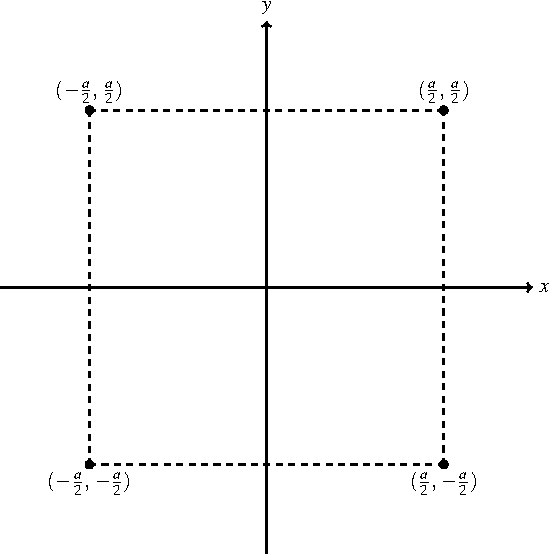
\includegraphics[scale=1.1]{image/03/square.pdf}
  \caption{%%
  }
  \label{fig:square_four_corners}
  \end{figure}
  \end{solution}
}{}

\item Suppose you move the square from
  \Problem{prob:square_centre_origin} by $b \geq 0$ units to the right
  and $b$ units upward.  Determine the new coordinates of each of the
  four corners of the square and the new coordinates of the centre.
\ifbool{showSolution}{
  \begin{solution}
  See \Figure{fig:square_shifted}.
  %%
  \begin{figure}[!htbp]
  \centering
  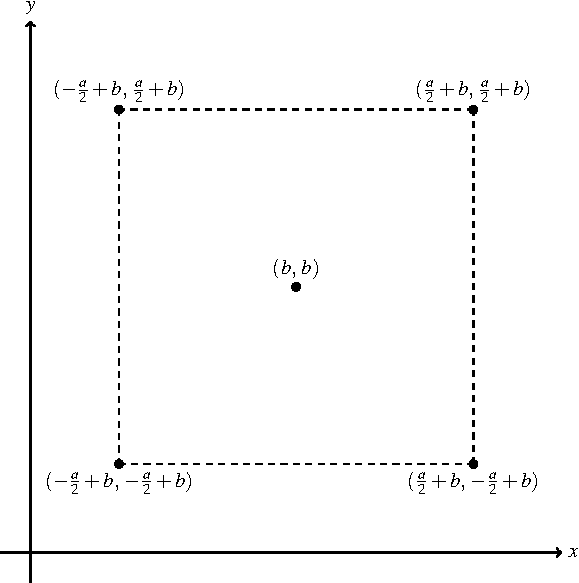
\includegraphics[scale=1.1]{image/03/square-shifted.pdf}
  \caption{%%
    The square from \Problem{prob:square_centre_origin} shifted by
    $b \geq 0$ units to the right and $b$ units upward.  The four
    corners of the square and the centre are shifted by $b$ units
    horizontally and vertically.
  }
  \label{fig:square_shifted}
  \end{figure}
  \end{solution}
}{}
\end{problem}

\end{document}
